%% PI-AI-MM manuscript -- Nature Article format (restructured 2026-11-10). Submission folder: paper/manuscript/main (self-contained).
%% Layout follows the Nature formatting guide: title <= 75 characters, referenced summary paragraph <= 200 words, unheaded
%% introduction, subheadings <= 40 characters, continuous prose, 5 main display items (Figs 1-4, Table 1), Methods with
%% Data/Code availability and the LLM statement, then references, end notes and Extended Data (1 figure, 7 tables).
%% Options: referee = double spacing, lineno = line numbers (both required for a PDF submission).
%% tables/ and figures/ are copies of paper/tables and paper/figures; refresh with: python refresh_from_package.py
%% Remaining author-only items are marked \todo{...}; disclosures are collected in disclosures/.

%% Page design: nature-style.tex (shared with supplementary.tex). This file builds the clean reading copy;
%% manuscript_submission.tex builds the same text double-spaced with line numbers for the Nature submission system.
\documentclass[11pt,a4paper]{article}
\input{nature-style}

\begin{document}
\pagestyle{plain}

\begin{flushleft}
{\sffamily\bfseries\fontsize{19}{23}\selectfont Reliability beyond accuracy in machine learning of magnetic materials\par}
\vspace{12pt}
{\sffamily\large Mujahidul Islam$^{1\,\ast}$ and Gayan P.~Hettiarachchi$^{1}$\par}
\vspace{6pt}
{\sffamily\footnotesize $^{1}$Digital Business and Innovation, Tokyo International University, 4-42-31 Higashi-Ikebukuro, Tokyo 170-0013, Japan.
$^{\ast}$e-mail: \href{mailto:mujahidmahfuz@gmail.com}{mujahidmahfuz@gmail.com}\par}
\end{flushleft}
\vspace{6pt}

%% Summary paragraph (Nature: bold first paragraph, fully referenced, ideally <= 200 words, written for non-specialists).
{\bfseries\noindent Machine learning is widely used to search for magnetic materials, which underpin electric motors, generators and data storage\cite{gutfleisch2011magnetic,coey2010magnetism}. Models trained on computed and literature-mined databases now predict magnetic ordering and the Curie temperature from chemical composition alone, and are usually judged by accuracy on held-out data\cite{nelson2019curie,long2021ferro,merker2022classifiers,itani2025nemad}. Whether such accuracy implies that added physical descriptors carry information, that stated uncertainties can be trusted or that predictions hold for unfamiliar chemistry is rarely tested\cite{meredig2018extrapolation,tran2020uq,kapoor2023leakage}. Here we show, on one curated dataset of about 79,000 ordering labels, 30,000 Curie temperatures and 88,000 computed moments, that these four properties are distinct. Descriptors from density functional theory gave no detectable gain over composition for ordering or the Curie temperature, and a small gain for the magnetic moment was mostly an effect of cell size. Prediction intervals were calibrated on average but failed for the highest predictions, and for antiferromagnets and ferrimagnets, unless the method was chosen with care. Ordering labels from computation and from experiment agreed no better than chance. On an audited external benchmark, error grew with chemical distance from the training data. Models intended for materials discovery should therefore be assessed on descriptor gains, calibration and transfer separately, in addition to accuracy.\par}
\vspace{8pt}

%% ===================================================================================================================
%% Introduction (no heading in Nature Articles)

High-throughput density functional theory (DFT) databases\cite{jain2013materials,saal2013oqmd,kirklin2015oqmd,choudhary2020jarvis,curtarolo2012aflow}, text-mined literature databases\cite{kelly2025curie,court2020phase,itani2025nemad} and curated magnetic-structure collections\cite{gallego2016magndata,gallego2016magndata2} have made it possible to train machine-learning models of magnetic ordering and of the Curie temperature \Tc{}. Composition-based models report \Tc{} errors of 56--69~K and ordering accuracies of 78--91\% on random or stratified splits\cite{nelson2019curie,long2021ferro,belot2023curie,merker2022classifiers,itani2025nemad,abediorang2026curie}. Structure-based graph networks\cite{merker2022classifiers,choudhary2021alignn} and high-throughput DFT\cite{horton2019ordering,frey2020oxides} offer other routes (Supplementary Table~9). None of the studies we examined evaluated on chemistry-grouped or provenance-shifted test sets, and the one cross-dataset test we found raised the \Tc{} error from 69 to 90~K\cite{belot2023curie}.

Accuracy on such splits is necessary but not sufficient. Work elsewhere in materials informatics has shown that random splits overstate extrapolation\cite{meredig2018extrapolation,xiong2020forwardcv,li2023critical,li2024mdhit,omee2024ood}, that accuracy on a proxy target need not carry over to the downstream task\cite{bartel2020stability}, that uncertainty estimates need separate validation\cite{tran2020uq,varivoda2023uq,palmer2022calibration} and that leakage inflates reported performance\cite{kapoor2023leakage,dunn2020matbench}. Methods exist for distribution shift\cite{koh2021wilds,tibshirani2019covariate} and for selective prediction\cite{geifman2017selective}, and active learning depends on uncertainty being usable\cite{lookman2019active}. For magnetic materials, however, no single study has measured descriptor gains, calibration and transfer on the same data and models, with resampling at the level at which records are dependent.

We did so for three targets: magnetic ordering, \Tc{} and the DFT magnetic moment. We asked three questions. Do DFT descriptors add information beyond composition? Are the uncertainties calibrated, both overall and for subgroups? Do predictions transfer to unfamiliar chemistry and to labels from another source? The answers differ by question. Several errors that we found in our own earlier analyses (Methods) show how easily each question can be answered wrongly.

%% ===================================================================================================================
\section*{Dataset and composition baselines}\label{sec:dataset}

We merged nine files from seven providers into one schema with row-level provenance (507,828 rows; Methods): Materials Project\cite{jain2013materials}, OQMD\cite{saal2013oqmd}, JARVIS-DFT\cite{choudhary2020jarvis}, two NEMAD releases\cite{itani2025nemad}, the ChemDataExtractor Curie/N\'eel database\cite{kelly2025curie}, MAGNDATA\cite{gallego2016magndata} and two experimental literature compilations. Written curation rules, which only remove rows, defined the targets (Table~\ref{tab:table1_dataset}). Two removals were large. Five rules took superconducting, ferroelectric and N\'eel temperatures and out-of-range values out of the text-mined `Curie temperature' column, which reduced it from 34,322 to 29,740 records. All 15,493 JARVIS ordering labels were quarantined, because they were a constant `ferromagnetic' returned by a data-collector default and not an assignment. The moment target is the DFT total magnetic moment of the computed cell at 0~K (\mcell{}), not an experimental saturation magnetization. Because \mcell{} grows with the number of atoms in the cell, we also analysed the moment per formula unit (\mfu{}).

Even after curation the \Tc{} labels are noisy. A title-based screen of 200 random curated records flagged 11.0\% (95\% interval 7.4--16.1\%) as likely wrong, mostly from the text-mined source (Supplementary Table~5). The median standard deviation of \Tc{} within a formula is 4.2~K, but 13\% of formulas with repeated records spread by more than 100~K.

Predictors form three nested tiers. Tier~1 holds 65 composition-only descriptors. Tier~2 adds 8 oxidation-state descriptors. Tier~3 adds 24 non-magnetic DFT descriptors of the most stable computed polymorph of each formula, such as formation energy, band gap, symmetry, volume, density and elastic and dielectric constants (Methods); it is available for 28,512 materials. DFT magnetic outputs were kept out of Tier~3 because they are the source of the moment labels and of part of the ordering labels, so including them would leak the label. All splits group records by reduced formula.

\begin{table}[h]
\caption{Prediction targets of the curated analysis dataset}
\label{tab:table1_dataset}
\begin{tabular*}{\textwidth}{@{\extracolsep\fill}llllll}
\toprule
Target & Unit & Records & Formulas & Train / validation / test & Matched Tier 1/2/3 records \\
\midrule
Magnetic ordering (FM/AFM/FiM/NM) & class & 79,125 & 70,293 & 55,249/11,974/11,902 & 6,061 \\
Curie temperature & K & 29,740 & 14,145 & 20,508/4,691/4,541 & 4,602 \\
DFT total magnetic moment per unit cell (Ms) & $\mu_\mathrm{B}$/cell & 87,513 & 77,402 & 61,254/13,130/13,129 & 10,852 \\
Mass magnetization (secondary) & emu/g & 4,317 & 3,218 & 3,021/648/648 & - \\
Volume magnetization (secondary) & A/m & 779 & 454 & 535/124/120 & - \\
Anisotropy constant K1 (secondary) & J/m$^3$ & 1,847 & 1,182 & 1,296/280/271 & - \\
\botrule
\end{tabular*}
\footnotetext{Analysis dataset v1.4 (frozen); formula-grouped 70/15/15 splits. Ordering classes: FM 34,098, NM 31,673, FiM 7,161, AFM 6,193. Tier 1 = 65 composition descriptors; Tier 2 = Tier 1 + 8 oxidation-chemistry descriptors; Tier 3 = Tier 2 + DFT physics descriptors (97 in total).}
\end{table}


Within the training distribution, composition alone was accurate. For ordering, XGBoost\cite{chen2016xgboost} reached a macro-F1 of 0.727 (0.711--0.744), against 0.469 for multinomial logistic regression and 0.151 for the majority class. For \Tc{}, gradient boosting\cite{ke2017lightgbm,pedregosa2011sklearn} reached a mean absolute error (MAE) of 76.2~K (69.9--82.5~K; $R^2$ 0.78), against 147.2~K for Ridge regression and 218.8~K for the training mean. For \mcell{}, gradient boosting reached 2.58~\muB{}/cell ($R^2\approx0.70$). Easy non-magnetic compounds do not drive the ordering score: restricting the test set to compounds that contain a magnetism-capable element lowered macro-F1 only from 0.692 to 0.681 over ten splits. Recall for antiferromagnets (AFM) and ferrimagnets (FiM) stayed near 0.55 and 0.49 (Supplementary Table~7).

%% ===================================================================================================================
\section*{Computed descriptors add little}\label{sec:rq1}

To test whether DFT descriptors add information, we compared the tiers on matched populations. These are the materials with complete Tier~3 descriptors, used with identical rows, splits, hyperparameter grids and metrics at every tier, over ten prespecified formula-grouped splits (Fig.~\ref{fig:rq1}, Extended Data Table~\ref{tab:table2_physics_descriptors}). We call a difference stable only if a refit-aware interval\cite{nadeau2003inference} and a formula-bootstrap interval both exclude zero and at least seven of the ten splits agree in sign. The nine Tier~1 to Tier~3 contrasts form the primary family and are Holm-corrected\cite{holm1979simple} (Methods).

For ordering and \Tc{}, no algorithm showed a stable Tier~2 or Tier~3 effect, and every primary adjusted $P$ value was 1.0. For \Tc{} the Tier~3 point estimates were losses: $-14.3$~K ($-42.5$ to $+13.9$) for gradient boosting, $-8.2$~K ($-48.3$ to $+32.0$) for XGBoost and $-14.4$~K ($-33.5$ to $+4.8$) for Ridge regression with clipped inputs. The design can detect only effects of about 40~K, and the intervals cannot exclude gains of 14--32~K, so we report no detectable gain and not the absence of a gain. The matched \Tc{} population is also much harder than the full one (Tier~1 MAE 203~K against 76~K), so the conclusion applies to materials with a full DFT record.

For \mcell{}, Tier~3 gave stable but small gains: $+0.079$~\muB{}/cell ($+0.030$ to $+0.127$) for gradient boosting and $+0.062$ ($+0.023$ to $+0.101$) for XGBoost, which is 2--3\% of the MAE (adjusted $P=0.046$). One scalar, the number of sites in the DFT cell, recovered about 70\% of the gradient-boosting gain when added to Tier~2, and what Tier~3 added beyond it was not resolved ($+0.024$; $-0.003$ to $+0.050$). The moment per formula unit behaved in the same way: gains were stable for all three algorithms ($+0.031$~\muB{} per formula unit for gradient boosting; $+0.014$ to $+0.048$), but beyond the site count they were no longer resolved for the tree models (Supplementary Table~8). Dividing the moment by the number of sites removes cell size directly, and a gain of about 3\% of the MAE remained for the tree models ($+2.9\%$ for gradient boosting, $+2.8\%$ for XGBoost) and 6.0\% for Ridge regression. The moment gain is therefore real but small, and mostly a cell-size effect.

\begin{figure}[t]
\centering
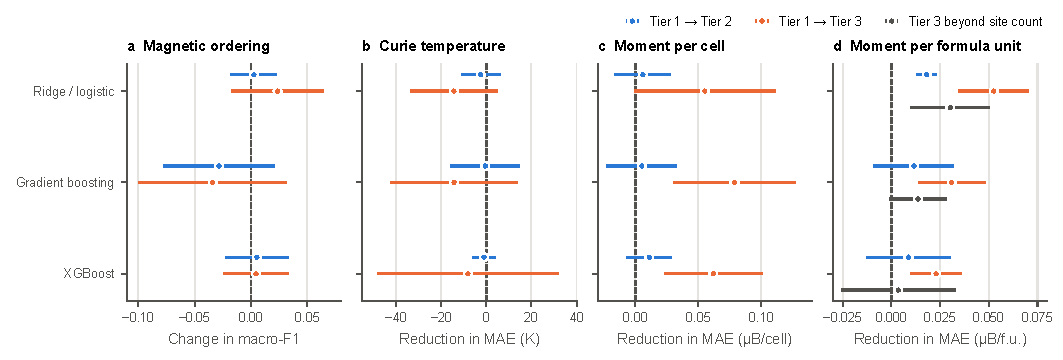
\includegraphics[width=\textwidth]{figures/fig1_physics_descriptors.pdf}
\caption{\textbf{Non-magnetic DFT descriptors add little beyond composition.} Change in test performance from Tier~1 (composition) to Tier~2 (oxidation state) and to Tier~3 (non-magnetic DFT descriptors) on identical matched materials. Points are means over ten prespecified formula-grouped splits and bars are refit-aware (Nadeau--Bengio) 95\% intervals; positive values are improvements. \textbf{a}, Macro-F1 for magnetic ordering. \textbf{b}, MAE for the Curie temperature (Ridge regression with clipped inputs). \textbf{c}, MAE for the DFT moment per cell. \textbf{d}, MAE for the DFT moment per formula unit, including the Tier~3 effect beyond a single site-count descriptor. XGBoost values in \textbf{b} and \textbf{c} are means of eight realizations.}\label{fig:rq1}
\end{figure}

A null result could reflect the choice of descriptors, because Tier~3 contains no magnetic quantities. For \Tc{}, where DFT magnetic quantities cannot leak the label, we therefore added three kinds of physics to the matched population (Extended Data Table~\ref{tab:table3_magnetic_physics}): ten magnetic-sublattice descriptors computed from the crystal structure, including the metal--anion--metal angles that govern superexchange; four DFT magnetic outputs; and a frozen 64-dimensional crystal embedding from the pretrained interatomic potential CHGNet. None improved on composition alone. Against Tier~1, the estimates ranged from $-10.8$ to $+9.5$~K and all intervals included zero. Relative to Tier~3, the embedding gave a stable $+19.2$~K for XGBoost and the magnetic outputs a borderline $+19.6$~K for gradient boosting; both roughly recover the Tier~3 loss and neither exceeds Tier~1.

Feature attribution did not reveal this. TreeSHAP\cite{lundberg2017shap,lundberg2020treeshap} assigned 40\% (ordering) and 36\% (\Tc{}) of the mean absolute attribution of Tier~3 XGBoost models to DFT descriptors that did not improve accuracy. Correlated composition and DFT features can carry the same information, so attribution shows that a feature is used, not that it adds value.

%% ===================================================================================================================
\section*{Calibration hides subgroup failures}\label{sec:rq2}

We next asked whether the uncertainties can be trusted. For regression we compared three conformal methods\cite{vovk2005algorithmic,lei2018distribution,angelopoulos2023gentle} at 90\% nominal coverage: constant-width split conformal prediction, normalized conformal prediction scaled by a learned difficulty model\cite{papadopoulos2011normalized}, and conformalized quantile regression\cite{romano2019cqr} (Fig.~\ref{fig:rq2}a,b, Extended Data Table~\ref{tab:table4_regression_intervals}). All three met 90\% coverage on average, as the theory guarantees: 89.3\%, 90.3\% and 89.4\% for \Tc{}, and 90.0--90.1\% for \mcell{}.

They differed for subgroups, which we defined independently of any method's difficulty score. In the top decile of predicted \Tc{}, normalized conformal prediction covered 87.4\%, split conformal 65.5\% and quantile regression 68.6\%. For text-mined labels the figures were 86.0\% against 78--79\%, and for the highest predicted third of \mcell{} 86.7\% against 72.3\% and 83.4\%. The normalized method was not better everywhere. On several chemical families and on the two curated Curie sources, the constant-width methods covered more (92--97\% against 89--92\%), because their intervals are wide everywhere (Supplementary Table~11). The normalized method was also more stable: its \Tc{} coverage varied between splits with a standard deviation of 2.5 points, against about 6 points for the other two. Records of one formula are dependent, so about 4,200 calibration rows act like only 250--340 independent ones (Supplementary Table~6).

Coverage was not protected against shift. It fell to 86.6--89.7\% in the decile farthest from the training chemistry, where calibrating separately for each distance quartile restored it (from 88.2\% to 90.3\%). When intervals were calibrated on curated rows and tested on text-mined rows, \Tc{} coverage was 76.9\% (split), 80.3\% (quantile) and 85.1\% (normalized).

The ordering classifier was trained with balanced class weights, so its raw probabilities follow a uniform prior. Correcting them to the training prior\cite{saerens2002adjusting} alone worsened the expected calibration error from 0.064 to 0.090, and adding temperature scaling\cite{guo2017calibration} reduced it to 0.014 (Extended Data Table~\ref{tab:table5_ordering_calibration}). Marginal conformal prediction sets met 90\% coverage overall (89.8\%) by over-covering ferromagnets (96.2\%) and non-magnets (97.7\%), while covering antiferromagnets 57.0\% and ferrimagnets 54.3\% of the time (Fig.~\ref{fig:rq2}c). Class-conditional sets\cite{vovk2013conditional} covered 89.8--90.9\% of every class, at a mean set size of 1.61 classes against 1.39.

\begin{figure}[t]
\centering
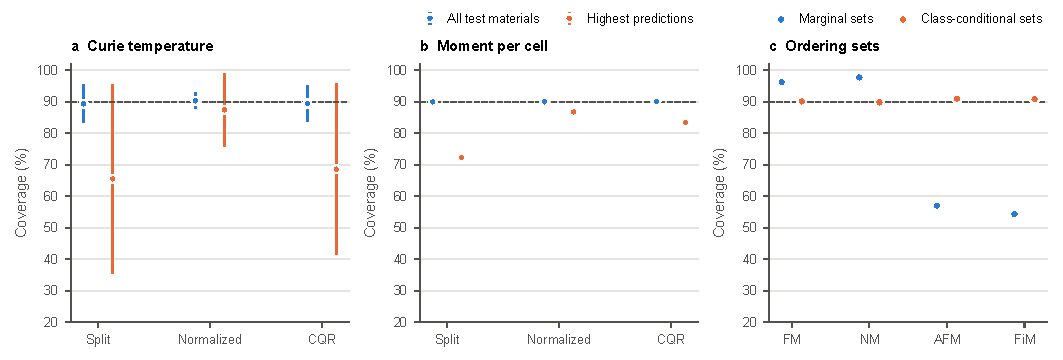
\includegraphics[width=\textwidth]{figures/fig2_uncertainty_calibration.pdf}
\caption{\textbf{Average coverage hides subgroup failures.} \textbf{a},\textbf{b}, Coverage of 90\% prediction intervals for the Curie temperature (\textbf{a}) and the DFT moment per cell (\textbf{b}), for all test materials and for the highest predictions (top decile in \textbf{a}, top third in \textbf{b}), under split, normalized and quantile (CQR) conformal prediction. Points are means over ten prespecified splits and bars are $\pm1$ s.d.\ across splits. \textbf{c}, Coverage of 90\% ordering prediction sets for each class (FM, ferromagnet; NM, non-magnet; AFM, antiferromagnet; FiM, ferrimagnet), for marginal and class-conditional sets, with temperature and thresholds fitted on separate halves of the calibration set. Dashed lines mark nominal coverage.}\label{fig:rq2}
\end{figure}

%% ===================================================================================================================
\section*{Ordering labels depend on provenance}\label{sec:provenance}

Of 949 formulas labelled by both Materials Project and an experimental source, the two labels agreed 28\% of the time, with Cohen's $\kappa=0.00$ ($-0.03$ to $0.03$): no better than chance. For 336 of 508 experimental antiferromagnets (66\%), the Materials Project label is ferromagnetic. This is consistent with high-throughput workflows that start from ferromagnetic configurations and enumerate antiferromagnetic orderings only for a subset\cite{horton2019ordering}.

Models did not bridge this gap (Extended Data Table~\ref{tab:table7_generalization_internal}). Trained on Materials Project labels and tested on experimental labels, the balanced accuracy was 0.337 (0.273--0.396). This is indistinguishable from models trained on permuted labels (median 0.342) and far below the 0.769 of a model trained on experimental labels; antiferromagnet recall was 7\%. In the reverse direction the balanced accuracy was 0.384 (0.366--0.401), just above the 97.5th percentile of the permuted-label models (0.351) and far below the within-source value of 0.591. The test compositions were not unusually far from the training compositions: the median composition distance to the nearest training formula was 0.081 across provenances, against 0.077 within Materials Project. The failure is therefore one of label definition, not of chemistry. A pooled ordering score measures agreement with a labelling convention as much as an ability to predict magnetic order.

%% ===================================================================================================================
\section*{Transfer to unfamiliar chemistry}\label{sec:rq3}

Within our data, holding out whole chemical systems (element sets) instead of formulas lowered ordering macro-F1 from 0.712 to 0.684 ($-0.028$; $-0.041$ to $-0.016$; worse in all ten paired splits), with ferrimagnet recall falling most (Extended Data Table~\ref{tab:table7_generalization_internal}). The moment degraded slightly but not stably ($+0.073$~\muB{}/cell; $-0.009$ to $+0.154$), and the change in \Tc{} error could not be resolved ($+2.7$~K; $-16.8$ to $+22.2$).

For an external test, we scored the Tier~1 XGBoost \Tc{} model and its normalized conformal intervals, without retraining or tuning, on an independent public table of 2,500 experimental Curie temperatures curated for a separate study\cite{malaei_magnetic_data,abediorang2026curie}. An audit came first (Methods; Supplementary Table~1). By composition, not by formula string, 1,998 records (80\%) were already in our repository, and 1,200 (48\%) carried a value identical to within 0.5~K to one we held. On those records the model scored $R^2$ 0.90, which reflects recall of training labels. After the exclusion of 105 records for stated reasons, 2,395 remained, of which 465 were compositions that the model had never seen.

On these 465 blind records, from 81 source-paper clusters, the MAE was 102.7~K (75.1--143.6~K) and $R^2$ was 0.69 (0.43--0.82), with interval coverage of 89.5\% (Fig.~\ref{fig:rq3}, Extended Data Table~\ref{tab:table6_external_benchmark}). Blind compositions in chemical systems that occur in the training data scored an MAE of 90.6~K and $R^2$ 0.78. The 69 records in unseen chemical systems, from only 18 clusters, scored an MAE of 171.9~K (82.6--293.7~K) and $R^2$ $-0.17$ ($-1.02$ to $0.64$). With chemical systems as the resampling unit, the upper limit of $R^2$ is 0.21 (Supplementary Table~4). We therefore state the conservative reading: in unseen chemical systems, the model's skill is not established.

\begin{figure}[t]
\centering
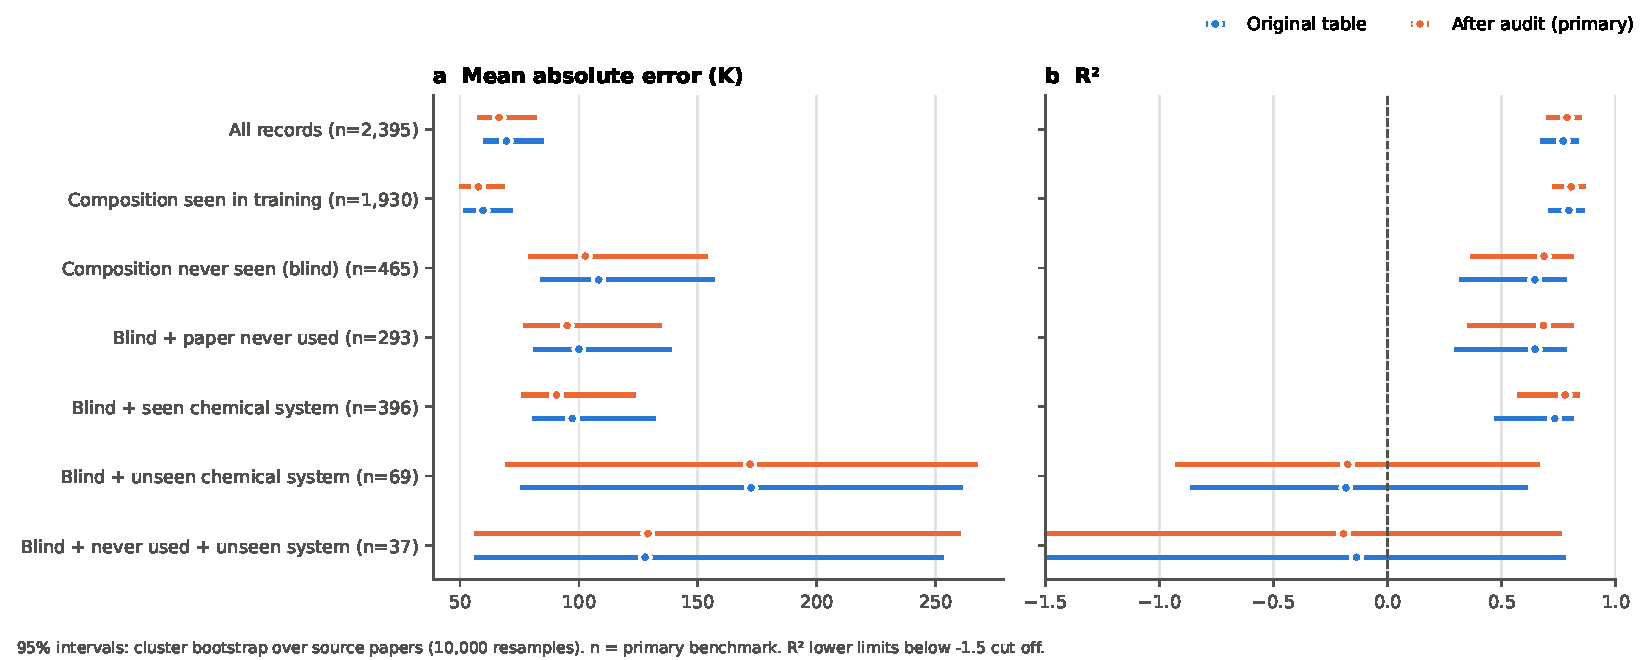
\includegraphics[width=\textwidth]{figures/fig3_external_benchmark.pdf}
\caption{\textbf{External benchmark of experimental Curie temperatures.} MAE (\textbf{a}) and $R^2$ (\textbf{b}) for nested novelty subsets of the external table, before and after the audit. Bars are 95\% intervals from a bootstrap over source-paper clusters (10,000 resamples); $n$ is the number of records after the audit, and lower limits of $R^2$ below $-1.5$ are cut off. `Blind' means that the composition never occurs in the training repository; `unseen system' means that its set of elements never occurs either.}\label{fig:rq3}
\end{figure}

Error depended on a similarity measure that we fixed in advance: the composition distance to the nearest training formula. On the blind records, error rose with distance (Spearman $\rho=0.28$; 0.10--0.49), and the MAE grew from 62~K in the closest quartile to 165~K in the farthest (Fig.~\ref{fig:distance}, Extended Data Fig.~\ref{fig:edscatter}). The normalized intervals widened, from 388 to 529~K, but not enough: coverage fell from 0.95 to 0.85 (Supplementary Table~3). Distance explains only part of the unseen-system result, because blind records in seen systems at comparable distance kept $R^2$ 0.75.

\begin{figure}[t]
\centering
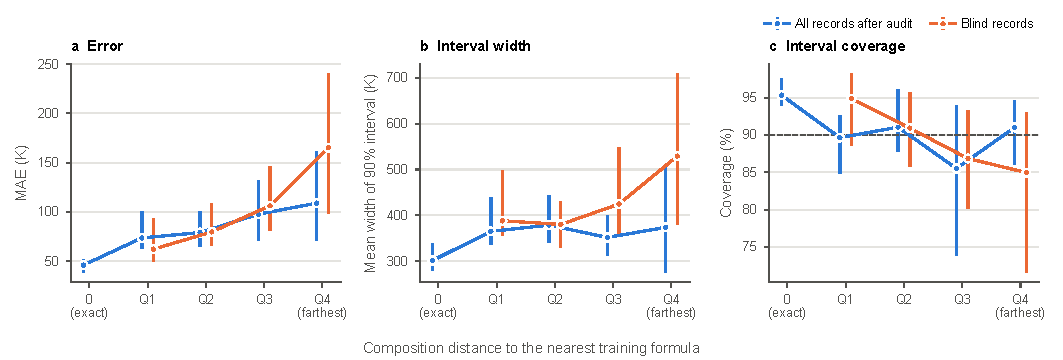
\includegraphics[width=\textwidth]{figures/fig4_error_vs_distance.pdf}
\caption{\textbf{Error grows and coverage falls with distance from the training chemistry.} External records binned by composition distance to the nearest training formula (bin 0, identical composition; Q1--Q4, quartiles of the non-zero distances), for all records after the audit and for the 465 blind records. \textbf{a}, MAE. \textbf{b}, Mean width of the 90\% interval. \textbf{c}, Coverage of the 90\% interval; the dashed line marks nominal coverage. Bars are 95\% paper-cluster bootstrap intervals.}\label{fig:distance}
\end{figure}

%% ===================================================================================================================
\section*{Use as a first screening filter}\label{sec:screening}

What do such predictions support in practice? On the 465 blind records, abstaining on the 50\% most distant compositions lowered the MAE from 103 to 71~K and raised coverage to 0.93 (Extended Data Table~\ref{tab:table8_screening}). Abstaining on interval width lowered the error similarly but did not raise coverage, so distance is the better abstention signal. For a room-temperature screen (\Tc{} above 300~K; base rate 0.57), the point prediction had a recall of 0.94 and a precision of 0.77. Deciding only when the 90\% interval lay wholly above or below 300~K settled 37\% of the records, with 92.5\% accuracy. The intervals are too wide to rank candidates within a family, but distance-based abstention and interval-based decisions make the model usable as a first filter.

%% ===================================================================================================================
\section*{Discussion}\label{sec:discussion}

The four properties that we measured are related, but none can be read off another. Composition-only models were accurate, yet DFT descriptors gave no detectable gain while receiving more than a third of the attribution. The most accurate ordering model needed prior correction and temperature scaling to be calibrated, and its marginal prediction sets covered antiferromagnets and ferrimagnets little more than half the time. Intervals that were calibrated overall lost coverage with chemical distance and under a change of label source. A \Tc{} model with $R^2$ 0.78 inside the training distribution has no established skill in unseen chemical systems, and an ordering model with macro-F1 0.73 transfers poorly between computed and experimental labels because the labels themselves disagree. Some of these outcomes were expected in principle: marginal conformal guarantees do not cover subgroups, and balanced class weights distort probabilities. What we add is their size for magnetic materials, and which simple remedies work.

Why did DFT descriptors not help? Our data favour two explanations. First, the DFT values describe the lowest-energy computed polymorph of a formula, whereas an experimental \Tc{} may refer to another structure, a doped sample or a film. The Tier~3 point estimates for \Tc{} were losses, as such a noisy join would produce, although we did not test this directly. Second, composition already fixes much of what the scalar descriptors encode. Where a gain appeared, it traced back to cell size. The null result is therefore narrow. It concerns descriptors joined by formula and used by tabular tree and linear models, together with one frozen embedding. It is not evidence against models that learn structure--property coupling from the measured phase end to end.

The study has limits. The external benchmark overlaps heavily with our sources, and the unseen-system conclusion rests on 69 records from 18 paper clusters. The label-noise screen was judged from titles by an AI assistant, so the 11\% figure is an estimate and not a verified error rate. Formula-grouped splits are not perfectly disjoint: formulas spelled in two ways affect 0.6\% of \Tc{} and 1.3\% of ordering test rows. The magnetic-physics test covers \Tc{} only, and we did not test end-to-end graph networks (Methods).

Several practices follow for evaluation. Descriptor sets should be compared on identical rows and repeated grouped splits, with a refit-aware interval and a simple size control. Coverage should be reported for subgroups that are defined independently of the uncertainty method. Novelty should be defined by composition and chemical system, and external test values checked against the training labels. Resampling should follow the dependence structure of the records, and data collectors should be audited for default values and labels for agreement across sources. For deployment, our results favour normalized or class-conditional conformal prediction, abstention far from the training data, and recalibration when the label source changes. In discovery the candidates are by definition unfamiliar. A model for discovery should therefore be judged by its behaviour away from the training data and by whether its uncertainty supports a decision, and not by in-distribution accuracy alone.

%% ===================================================================================================================
\section*{Methods}\label{sec:methods}

\subsection*{Data collection and harmonization}
The sources were: Materials Project\cite{jain2013materials} (100,000 entries, with ordering, total magnetization and summary properties retrieved through the API); OQMD\cite{saal2013oqmd,kirklin2015oqmd}, via jarvis-tools; JARVIS-DFT\cite{choudhary2020jarvis} (entries with a moment above 0.05~\muB{}); NEMAD\cite{itani2025nemad}; the ChemDataExtractor Curie/N\'eel database of Kelly and Cole\cite{kelly2025curie}; MAGNDATA\cite{gallego2016magndata,gallego2016magndata2}; and two experimental literature compilations of magnetic and anisotropy properties, of undocumented provenance (Data availability). Sources were mapped to a 25-column schema. Each property kept its value, unit and measurement temperature, and each row kept its source file. Records were deduplicated on material name plus DOI, so independent measurements of one composition were kept (507,828 rows). Formulas were canonicalized with pymatgen\cite{ong2013pymatgen}, and 1,940 records with non-chemical `formulas' (trade names and generic templates such as ABO$_3$) were quarantined.

\subsection*{Descriptors}
Tier~1 (65 descriptors) holds composition statistics in the spirit of Magpie\cite{ward2016magpie}: element flags and fractions; transition-metal, rare-earth, actinide and magnetic-element fractions; $s$, $p$, $d$ and $f$ fractions and counts of unpaired, $d$ and $f$ electrons; valence-electron concentration; means and variances of radius, electronegativity, mass, melting temperature, period and group; and size mismatch and entropies. Tier~2 adds eight oxidation-state statistics from pymatgen's charge-balancing guesser. Tier~3 adds 24 non-magnetic DFT properties joined by reduced formula from the most stable polymorph: formation energy, energy above hull, band gap and band edges, Fermi level, space group, crystal system, point group, volume and density, elastic moduli, dielectric constants, refractive index and the maximum piezoelectric coefficient. Materials Project was the primary source; JARVIS provided elastic and dielectric tensors where denser, and AFLOW\cite{curtarolo2012aflow} provided thermal properties. Excluded by design were the magnetic flag, the number of magnetic sites, the magnetic species, total magnetization, magnetization per volume, the DFT ordering and the elastic tensor. The first six are close to the labels, and the elastic tensor is not a scalar. Four finite values that overflow single precision were set to missing.

\subsection*{Magnetic-physics test}
This test covers \Tc{} only. Structures were fetched for the same Materials Project entries (4,849 structures). Magnetic ions are the elements of curation rule C1 below, and bridging anions are O, S, Se, Te, N, P, As, F, Cl, Br and I. Ten sublattice descriptors were computed with pymatgen: the magnetic site fraction and density; the shortest and the mean nearest metal--metal (M--M) distance; the number of M neighbours within 1.15 times the nearest M--M distance; the mean nearest metal--anion (M--X) distance and the M coordination (X within 1.2 times the nearest distance); the mean M--X--M angle around each anion over its bonded M neighbours, including periodic images; and the fractions of those angles in [150,~180] and [80,~100] degrees. The code was checked on rock-salt MnO and cubic SrFeO$_3$. The DFT magnetic outputs were the moment per atom, the magnetic-site fraction, the magnetization per volume and the magnetic flag. The CHGNet embedding is the 64-dimensional pooled crystal feature of the pretrained model (chgnet 0.4.2), used without training. The revision plan also contained a comparison restricted to records whose source reports a space group equal to that of the computed polymorph. This comparison, and the same test for ordering and the moment, were dropped for run time before any of their results were seen (\texttt{results/revision/PLAN.md}, deviations log).

\subsection*{Targets and curation}
For ordering, 116 raw labels were mapped to ferromagnetic (FM), antiferromagnetic (AFM), ferrimagnetic (FiM) and non-magnetic (NM). Hedged labels (`ferromagnetic-like') and distinct states (spin glass, superparamagnet) were excluded. Compensated ferrimagnets were kept as FiM. All JARVIS rows were quarantined because their label was a collector constant.

Curie temperatures were converted to kelvin. Placeholder zeros of one source and 54 encoded values were removed. Five rules then removed records: C1, formulas without a magnetism-capable element; C2, single elements that are not ferromagnets; C3, values below 1~K; C4, values above 1,400~K, which is above the highest known ferromagnetic \Tc{}, that of Co at about 1,388~K\cite{coey2010magnetism}; and C5, formulas labelled only AFM in every source. These rules are screens with known false positives (for example YTiO$_3$, removed by C1). A sensitivity target without C5 gave the same baselines. The rules were written after the analyses of an earlier dataset version had been seen, and before any model was fitted on the curated target.

For the title-based screen, we drew a stratified random sample of 200 curated records (source by \Tc{} tercile, seed 20261110). Each record was classified from its Crossref title, compound and value, without reading the full paper, as a magnetic Curie transition, another transition, an implausible value, a computational source, a different compound, a film or nanoscale sample, or unclear. Of the 11.0\% flagged, 3.5\% were other transitions, 3.5\% implausible values and 4.0\% came from computational papers. The classification was made by the AI assistant (see Use of large language models) \todo{and checked by the authors on N records with M disagreements: complete after the spot check}. Some categories, notably `implausible value', involve judgement. The per-record labels are released so that they can be checked.

The moment \mcell{} is the Materials Project or JARVIS total moment of the computed cell at 0~K. Of the Materials Project entries, 98\% come from the mixed GGA/GGA+U scheme and 1\% from r$^2$SCAN alone. Their recorded orderings are 54\% FM, 27\% unknown, 9\% FiM, 7\% AFM and 4\% NM; most entries were computed from ferromagnetic initial configurations\cite{horton2019ordering}. The moment per formula unit is \mfu{} = \mcell{} $\times$ (atoms per formula unit)/(atoms in the cell), using the atom count of the same calculation (10,821 rows). Mass and volume magnetization and the anisotropy constant $K_1$ are secondary targets.

\subsection*{Splits, models and selection}
Records were split 70/15/15 by reduced formula with a size-balanced, stratified group assignment. StratifiedGroupKFold was not used because a few formulas with many records made it unbalanced. Robustness analyses used ten splits with prespecified seeds ($20267000+i$), and leave-chemical-system-out splits grouped records by element set. The models were multinomial logistic or Ridge regression with median imputation and standardization, histogram gradient boosting\cite{pedregosa2011sklearn,ke2017lightgbm} and XGBoost\cite{chen2016xgboost}; classifiers used balanced class weights. Hyperparameters were chosen on validation macro-F1 (classification) or root-mean-square error (regression), the model was refitted on training plus validation data, and it was scored once on the test set. The grids were $C\in\{0.1,1,10\}$ or $\alpha\in\{0.1,1,10,100\}$ for the linear models; 500 iterations, learning rate in $\{0.05,0.1\}$ and leaf nodes in $\{31,127\}$ for gradient boosting; and 500 trees, depth in $\{6,10\}$, learning rate in $\{0.05,0.1\}$ and subsample and column fractions of 0.8 for XGBoost. On the full populations, histogram gradient boosting reached an ordering macro-F1 of 0.720 and XGBoost a \Tc{} MAE of 75.4~K.

XGBoost results depend on the thread count, which acts like a random seed: the mean prediction changes by about 25\% of the MAE between settings. Tier results for \Tc{} and \mcell{} are therefore averaged over eight thread and seed realizations. Ordering XGBoost tier results come from one realization; gradient boosting, which does not depend on the thread count, gives the same conclusion. Unclipped Ridge regression produced exploded Tier~3 predictions from a few non-physical inputs (an elastic-anisotropy ratio of order $10^{110}$), so Ridge results for \Tc{} use clipped inputs.

\subsection*{Statistics}
Tier differences were computed on identical test materials. For each contrast we report the mean over the ten splits and two 95\% intervals: a pooled formula-bootstrap interval (1,000 resamples, with the same draws for both tiers), and a Nadeau--Bengio corrected resampled-$t$ interval, whose variance is inflated by $1/J+n_\mathrm{test}/n_\mathrm{train}$ for the overlap between the $J$ splits\cite{nadeau2003inference}. Tests are two-sided. A contrast is stable if both intervals exclude zero and at least seven of the ten splits agree in sign, and borderline if only one interval excludes zero. The nine Tier~1 to Tier~3 contrasts (three targets by three algorithms) form the primary family and are Holm-corrected\cite{holm1979simple}; all other contrasts are secondary. Practical margins were fixed before the revision analyses: 10~K for \Tc{}, 0.02 for macro-F1 and 0.10~\muB{}/cell. The minimum detectable effect is stated at 80\% power. Unless stated otherwise, ranges in parentheses in the main text are 95\% intervals.

Additional contrasts were as follows. For ordering, the gradient-boosting Tier~1 to Tier~2 loss ($-0.028$) was not stable under the refit-aware test. For \mfu{}, the Tier~3 gains were $+0.023$ for XGBoost and $+0.053$ for Ridge regression; beyond the site count, the gains were $+0.014$ ($-0.001$ to $+0.028$) for gradient boosting, $+0.004$ ($-0.026$ to $+0.033$) for XGBoost and a stable $+0.030$ ($+0.010$ to $+0.051$) for Ridge regression. The per-atom gains had across-split intervals of 1.5--4.4\% (gradient boosting), 1.6--3.9\% (XGBoost) and 5.1--6.8\% (Ridge regression). Earlier add-one analyses attributed the per-atom residual mainly to outputs of the same DFT calculation that produced the moment. TreeSHAP rankings were stable over ten splits for ordering and the moment (mean pairwise Spearman correlation of at least 0.95) but not for \Tc{} (0.83--0.94), so for \Tc{} we make statements about descriptor families only.

The Phase~7 comparisons were configured before their models were fitted. The revision analyses were planned in writing before they were run, and analyses dropped for run time were removed before their results were seen. Both documents are released (\texttt{results/revision/PLAN.md}).

\subsection*{Uncertainty quantification}
For regression intervals, whole formulas (20\% of the training formulas) formed the calibration set, and models were refitted on the remaining 80\%. Split conformal prediction used absolute residuals. Normalized conformal prediction divided them by a difficulty model fitted to cross-fitted absolute residuals. Conformalized quantile regression used XGBoost 5\% and 95\% quantile models. Subgroups for evaluation were defined without any method's difficulty score. The design effect is $1+(\bar m-1)\rho$, where $\rho$ is the within-formula intraclass correlation of the calibration exceedance indicator and $\bar m$ is the size-weighted formula size; it was 12--17, which predicts a split-to-split standard deviation of coverage of 1.6--1.9 points. This explains most of the variability of the normalized method but not the larger swings of the constant-width methods. Distance-aware (Mondrian) conformal prediction calibrates separately for each quartile of calibration distance. Weighted conformal prediction used a logistic density ratio of $\log(1+d)$\cite{tibshirani2019covariate}; it changed nothing, because calibration and test sets come from the same pool.

For ordering, probabilities were prior-corrected to the training prior\cite{saerens2002adjusting} and temperature-scaled on half of the calibration formulas. Marginal and class-conditional thresholds on $1-p_\mathrm{true}$ were set on the other half\cite{vovk2013conditional}; fitting both on the same half changed coverage by less than 0.3 points. Expected calibration error is reported for the top label and classwise\cite{kull2019dirichlet}, with 15 equal-width bins. Classwise error changed much less than top-label error (0.035 raw, 0.049 prior-corrected, 0.032 with temperature scaling), so temperature scaling fixes confidence and not the per-class probabilities. Sets calibrated on Materials Project labels and tested on experimental labels covered 83.5\%.

\subsection*{Cross-provenance ordering}
For formulas labelled by both Materials Project and an experimental source, we compared the modal label of each provenance (Cohen's $\kappa$, formula bootstrap). For transfer, NM was removed everywhere, because the experimental labels contain only five NM rows. Models were trained on one provenance, with training formulas present in the target test set removed and hyperparameters selected on the source validation rows, and were tested on the target test rows. The reported values use raw probabilities. A variant with probabilities prior-corrected to the target domain's training-partition prior gave balanced accuracies of 0.314 (0.247--0.381) from Materials Project to experimental labels and 0.400 (0.370--0.430) in the reverse direction, and does not change the conclusions. The null distribution came from 20 refits on permuted training labels; its 97.5th percentile was 0.374 for the Materials Project to experimental direction.

\subsection*{Leave-chemical-system-out test}
This test used fixed hyperparameters on ten random splits of the full populations, so its baselines (for example 99~K for \Tc{}) differ from the frozen-split values. The formula-grouped and system-grouped schemes test different materials, so the reported changes combine novelty with differences in test composition.

\subsection*{External benchmark and audit}
The external table\cite{malaei_magnetic_data,abediorang2026curie} lists 2,500 ferromagnets with experimental \Tc{} and source DOIs. It is not redistributed; a script downloads the analysed version and checks its SHA-256 hash. Audit checks A1--A8 (Supplementary Table~1) were written down before any record-level error was linked to an audit flag or a distance. They were written after the subset-level results of an earlier analysis were known; that analysis defined novelty by formula string and missed a DOI prefix (see below). Three amendments were logged, one of them (first-DOI clusters) after the first bootstrap run. The 105 excluded records comprised 60 computational labels, 18 malformed compositions and 35 values outside our target definition; some records fall under more than one reason.

Novelty uses composition identity and normalized DOIs. Distance is the total-variation distance between element-fraction vectors to the nearest of 23,757 training formulas. Clusters are records linked by any shared DOI (the prespecified unit), by first-listed DOIs or by chemical systems. Intervals are percentile and bias-corrected and accelerated cluster-bootstrap intervals (10,000 resamples). Skill is measured against a fixed training-mean predictor (\Tc{} = 338~K); for the unseen-system records it was $-0.17$ ($-0.77$ to $0.56$).

Before analysing the corrected subsets we fixed a wording rule: claim `no skill beyond the mean' only if the upper limit is at most 0.2. The rule was written after the subset results of the earlier, flawed analysis were known. With paper clusters, the rule gives `much weaker, with wide uncertainty'. With chemical systems as the resampling unit, the upper limits are 0.21 for $R^2$ and 0.17 for the fixed-reference skill. The screening analysis of the 465 blind records was added in revision.

\subsection*{Errors found and corrected}
During the study we found and corrected the following errors in our own work: a collector default `ferromagnetic' label on all JARVIS entries (16\% of an earlier ordering target); non-Curie transitions in a text-mined \Tc{} column; per-atom moments divided by the atom count of a different cell (25.4\% of rows); an external `blind' test that compared formula strings (1,302 claimed blind records against 502 by composition); a DOI normalizer that missed the \url{https://doi.org/} prefix; and a single-split Tier~2 ordering gain that did not replicate. In revision we corrected a stability rule described more loosely than implemented, a difficulty subgroup defined by the method under test, a three-class chance reference for a four-class predictor, paper counts reported instead of resampling clusters, and the wrong citation for the text-mined database. Earlier results are kept unchanged, and each correction is recorded in a versioned claims register.

\subsection*{Further limitations}
The matched leave-chemical-system-out comparison scores different test materials under the two schemes. Matched populations are harder than the full populations for \Tc{}, so the tier conclusions apply to materials with full DFT records. For the moment and for ordering, magnetic DFT outputs would leak the label, and we did not repeat the geometry and embedding test for them. We tested tabular tree and linear models and a frozen crystal embedding, not end-to-end graph networks. Within-formula spreads of \Tc{} above 100~K are common enough to limit any \Tc{} model.

\subsection*{Use of large language models}
The data pipeline, analyses and manuscript were developed with substantial assistance from a large language model (Claude, Anthropic), which wrote code, ran analyses, classified the records of the title-based screen and drafted text under the authors' direction. The authors checked the analyses and take full responsibility for the content. \todo{authors to confirm the extent of their checks before submission}

\subsection*{Data availability}
The curated analysis dataset (versions 1.2--1.4), frozen splits, external-benchmark adjudications, title-screen labels and all result files form the reproducibility package \todo{repository and DOI}. Redistribution follows the upstream terms (Supplementary Table~10). Derived values from Materials Project, OQMD, JARVIS-DFT, the Kelly--Cole database and the NEMAD Zenodo release are released under CC~BY~4.0 with attribution. AFLOW terms permit non-commercial use only, MAGNDATA has no public licence, and the two experimental compilations are of undocumented origin. The external benchmark table has no licence and is not redistributed; a script retrieves the analysed version and checks its SHA-256 hash. \todo{Before deposit: replace MAGNDATA, compilation and AFLOW values by identifiers plus retrieval scripts (or obtain permission), and drop the external compound names and values from the three result files that contain them.}

\subsection*{Code availability}
All analysis code, configurations with fixed seeds, table and figure builders and tests are in the reproducibility package, released under the MIT licence \todo{repository URL}. Run time is about 2--10 minutes per split for the tier and uncertainty analyses on a 16-thread workstation. XGBoost results reproduce exactly only at the same thread count.

%% ===================================================================================================================
%% Single reference list (main-text and Methods-only references are numbered in order of first appearance).
{\singlespacing
\bibliography{references}
}

\bmhead{Acknowledgements}
\todo{acknowledgements, or delete this section}

\bmhead{Funding}
\todo{state funding, or ``The authors received no specific funding for this work.''}

\bmhead{Author contributions}
\todo{confirm: M.I. conceived the study, curated the data, developed the methods and software, performed the analyses and wrote the first draft. G.P.H. supervised the work, contributed to the methods and revised the manuscript.}

\bmhead{Competing interests}
The authors declare no competing interests.

\bmhead{Additional information}
\textbf{Supplementary information} is available for this paper (Supplementary Tables~1--11 and reproducibility notes). \textbf{Correspondence and requests for materials} should be addressed to Mujahidul Islam.

%% ===================================================================================================================
%% Extended Data (online only; at most ten items). Counters restart so that items read "Extended Data Fig. 1", "Extended Data Table 1", ...
%% Each item is fixed in place ([H]) in the order of first citation, so nothing drifts.
\clearpage
\ifdefined\submissionmode\nolinenumbers\fi
\setcounter{figure}{0}
\setcounter{table}{0}
\renewcommand{\figurename}{Extended Data Fig.}
\renewcommand{\tablename}{Extended Data Table}
\renewcommand{\theHfigure}{ED\arabic{figure}}
\renewcommand{\theHtable}{ED\arabic{table}}
\floatplacement{table}{H}
\floatplacement{figure}{H}
\section*{Extended Data}

\begin{figure}
\centering
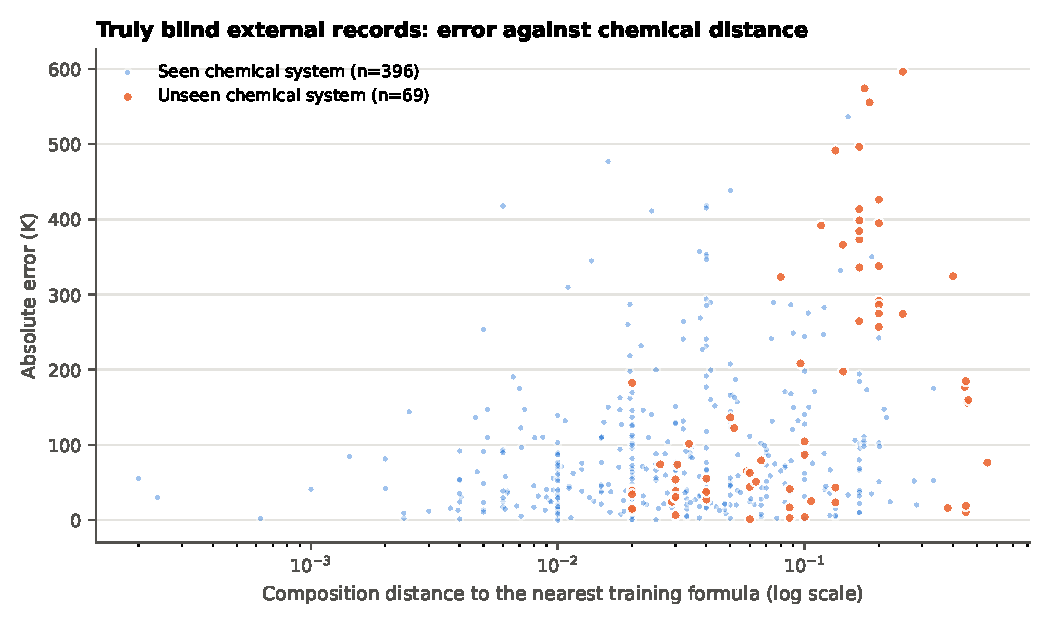
\includegraphics[width=120mm]{figures/figS1_blind_scatter.pdf}
\caption{\textbf{Error against chemical distance for every blind external record.} Absolute error of the Curie-temperature prediction against the composition distance to the nearest training formula (log scale) for the 465 blind records of the external benchmark. Records in unseen chemical systems are highlighted.}\label{fig:edscatter}
\end{figure}

\vspace{10pt}
\begin{table}[h]
\caption{Effect of oxidation-chemistry (Tier 2) and DFT physics (Tier 3) descriptors on matched populations}
\label{tab:table2_physics_descriptors}
\begin{tabular*}{\textwidth}{@{\extracolsep\fill}lllll}
\toprule
Target, metric & Algorithm & Tier 1$\rightarrow$2 & Tier 1$\rightarrow$3 & Tier 1$\rightarrow$3 verdict \\
\midrule
Curie temperature, MAE (K) & Gradient boosting & -0.4 [-9.6, +7.5] & -14.3 [-31.3, +3.8] & no meaningful improvement \\
Curie temperature, MAE (K) & Ridge / logistic & -3.6 [-11.0, +4.6] & -825.2 [-2938.0, +8.8] & no meaningful improvement \\
Curie temperature, MAE (K) & XGBoost & +1.1 [-5.9, +8.0] & -9.7 [-24.1, +3.5] & no meaningful improvement \\
Ms per atom, relative MAE gain (\%) & Gradient boosting & - & +2.9 [+1.5, +4.4] & stable gain \\
Ms per atom, relative MAE gain (\%) & Ridge / logistic & - & +6.0 [+5.1, +6.8] & stable gain \\
Ms per atom, relative MAE gain (\%) & XGBoost & - & +2.8 [+1.6, +3.9] & stable gain \\
Ms per cell, MAE ($\mu_\mathrm{B}$/cell) & Gradient boosting & +0.005 [-0.009, +0.021] & +0.079 [+0.049, +0.111] & stable improvement \\
Ms per cell, MAE ($\mu_\mathrm{B}$/cell) & Ridge / logistic & +0.006 [-0.003, +0.016] & +0.055 [+0.002, +0.099] & stable improvement \\
Ms per cell, MAE ($\mu_\mathrm{B}$/cell) & XGBoost & -0.004 [-0.021, +0.013] & +0.037 [-0.000, +0.072] & not stable \\
Ordering, macro-F1 & Gradient boosting & -0.029 [-0.057, -0.001] & -0.034 [-0.073, +0.002] & not stable \\
Ordering, macro-F1 & Ridge / logistic & +0.004 [-0.009, +0.019] & +0.024 [-0.008, +0.058] & not stable \\
Ordering, macro-F1 & XGBoost & +0.005 [-0.009, +0.019] & +0.005 [-0.024, +0.033] & not stable \\
\botrule
\end{tabular*}
\footnotetext{Improvement = Tier k minus Tier 1 performance, positive = better; identical rows, splits, grids and metrics at every tier; 10 repeated formula-grouped splits; 95\% intervals. Matched N: ordering 6,061, Curie 4,602, Ms 10,852 (per atom 10,821 after the denominator correction). Curie verdict uses a 10 K margin. Ridge Curie Tier 3 fits are numerically unstable (exploded predictions on a few rows). XGBoost results depend on the thread count; across thread/seed realisations the Ms per-cell XGBoost Tier 1$\rightarrow$3 gain ranges from +0.026 to +0.062 $\mu_\mathrm{B}$/cell.}
\end{table}

\clearpage
\begin{table}
\caption{Magnetic and structure-aware physics for the Curie temperature}
\label{tab:table3_magnetic_physics}
\tablefont
\begin{tabularx}{\textwidth}{@{}>{\raggedright\arraybackslash}Xrllll@{}}
\toprule
\textbf{Algorithm} & \textbf{MAE (K)} & \textbf{vs Tier 1} & \textbf{Verdict vs Tier 1} & \textbf{vs Tier 3} & \textbf{Verdict vs Tier 3} \\
\midrule
\multicolumn{6}{@{}l@{}}{\textit{Tier 1 + magnetic-sublattice geometry (10)}} \\
\quad Gradient boosting & 202.6 & +0.3 [$-$13.9, +14.5] & none & -- & -- \\
\quad XGBoost & 203.6 & +5.8 [$-$15.8, +27.4] & none & -- & -- \\
\addlinespace
\multicolumn{6}{@{}l@{}}{\textit{Tier 3 + magnetic-sublattice geometry}} \\
\quad Gradient boosting & 220.2 & -- & -- & $-$3.1 [$-$27.6, +21.4] & none \\
\quad XGBoost & 211.0 & -- & -- & +8.0 [$-$15.8, +31.9] & none \\
\addlinespace
\multicolumn{6}{@{}l@{}}{\textit{Tier 3 + DFT magnetic outputs (4)}} \\
\quad Gradient boosting & 197.6 & +5.3 [$-$29.9, +40.4] & none & +19.6 [$-$3.1, +42.3] & borderline gain \\
\quad XGBoost & 210.7 & $-$1.4 [$-$35.8, +33.0] & none & +8.3 [$-$27.5, +44.2] & none \\
\addlinespace
\multicolumn{6}{@{}l@{}}{\textit{Tier 3 + geometry + DFT magnetic outputs}} \\
\quad Gradient boosting & 205.6 & $-$2.8 [$-$39.1, +33.6] & none & +11.5 [$-$14.4, +37.4] & none \\
\quad XGBoost & 201.9 & +7.5 [$-$33.8, +48.8] & none & +17.2 [$-$9.5, +43.9] & borderline gain \\
\addlinespace
\multicolumn{6}{@{}l@{}}{\textit{Tier 3 + CHGNet crystal embedding (64)}} \\
\quad Gradient boosting & 213.7 & $-$10.8 [$-$22.5, +0.9] & none & +3.5 [$-$19.2, +26.2] & none \\
\quad XGBoost & 199.9 & +9.5 [$-$28.7, +47.7] & none & +19.2 [+0.4, +38.0] & stable gain \\
\bottomrule
\end{tabularx}
\par\vspace{4pt}\raggedright\noindent Matched Curie population (4,602 records), same 10 splits as Extended Data Table 1; MAE of Tier 1 / Tier 3: gradient boosting 202.9 / 217.1 K, XGBoost 209.3 / 219.1 K. Geometry: magnetic-ion site fraction and density, nearest and mean M-M distance, M-M connectivity, M-X distance and coordination, mean M-X-M angle and the fractions of angles in [150, 180] and [80, 100] degrees, from the Materials Project structure of the same entry. DFT magnetic outputs (moment per atom, magnetic-site fraction, magnetization per volume, magnetic flag) are not label leakage for experimental Curie temperatures. CHGNet = frozen 64-d crystal feature of the pretrained universal potential. Improvement in K, positive = better; Nadeau-Bengio 95\% intervals; verdict 'none' = no stable change; XGBoost single realization.
\end{table}

\vspace{10pt}
\begin{table}
\caption{Coverage of 90\% conformal prediction intervals, overall and in subgroups}
\label{tab:table4_regression_intervals}
\tablefont
\begin{tabularx}{\textwidth}{@{}>{\raggedright\arraybackslash}Xlllll@{}}
\toprule
\textbf{Method} & \textbf{All, mean (SD)} & \textbf{Mean width} & \textbf{High predictions} & \textbf{Second subgroup} & \textbf{Farthest distance decile} \\
\midrule
\multicolumn{6}{@{}l@{}}{\textit{Curie temperature}} \\
\quad Split conformal & 89.3 (6.0) & 569 K & top decile 65.5 & text-mined 78.2 & 86.6 \\
\quad Normalized conformal & 90.3 (2.5) & 451 K & top decile 87.4 & text-mined 86.0 & 88.2 \\
\quad CQR & 89.4 (5.8) & 519 K & top decile 68.6 & text-mined 79.3 & 89.7 \\
\addlinespace
\multicolumn{6}{@{}l@{}}{\textit{Moment per cell}} \\
\quad Split conformal & 90.0 (0.4) & 12.6 $\mu_\mathrm{B}$/cell & top third 72.3 & oxides 84.0 & -- \\
\quad Normalized conformal & 90.0 (0.5) & 11.7 $\mu_\mathrm{B}$/cell & top third 86.7 & oxides 91.0 & -- \\
\quad CQR & 90.1 (0.4) & 9.8 $\mu_\mathrm{B}$/cell & top third 83.4 & oxides 89.5 & -- \\
\bottomrule
\end{tabularx}
\par\vspace{4pt}\raggedright\noindent Nominal 90\%; 10 prespecified formula-grouped splits; calibration on 20\% of training formulas; coverage in \%. Subgroups are defined without any method's own difficulty score: top decile of the point prediction (Curie) or highest predicted third (moment), the text-mined label source (Curie) or oxides (moment), and the farthest decile of composition distance to the proper-training formulas. For comparison, on the decile defined by the normalized method's own difficulty scale (a circular definition used in an earlier analysis) coverage is 54/89/61\% for split/normalized/CQR (Curie).
\end{table}

\clearpage
\begin{table}
\caption{Calibration of magnetic-ordering probabilities and prediction sets}
\label{tab:table5_ordering_calibration}
\tablefont
\begin{tabularx}{\textwidth}{@{}>{\raggedright\arraybackslash}Xrrrrrrrr@{}}
\toprule
\textbf{Probabilities / sets} & \textbf{Top-label ECE} & \textbf{Classwise ECE} & \textbf{Coverage (\%)} & \textbf{FM} & \textbf{AFM} & \textbf{FiM} & \textbf{NM} & \textbf{Set size} \\
\midrule
raw (balanced-weight) probabilities & 0.064 & 0.035 & -- & -- & -- & -- & -- & -- \\
prior-corrected & 0.090 & 0.049 & -- & -- & -- & -- & -- & -- \\
prior-corrected + temperature & 0.014 & 0.032 & -- & -- & -- & -- & -- & -- \\
Class-conditional sets & -- & -- & 90.1 (0.6) & 90.1 & 90.9 & 90.8 & 89.8 & 1.61 \\
Marginal sets & -- & -- & 89.8 (0.9) & 96.2 & 57.0 & 54.3 & 97.7 & 1.39 \\
\bottomrule
\end{tabularx}
\par\vspace{4pt}\raggedright\noindent Mean over 10 prespecified splits (Tier 1 XGBoost, full ordering population); 15 equal-width bins. Sets at 90\% nominal on prior-corrected, temperature-scaled probabilities, with the temperature fitted on half of the calibration formulas and the conformal thresholds on the other half (re-using one calibration set gives the same coverage to within 0.3 points). Coverage = mean (SD).
\end{table}

\vspace{10pt}
\begin{table}
\caption{Generalization to unfamiliar chemical systems and to another label provenance}
\label{tab:table7_generalization_internal}
\tablefont
\begin{tabularx}{\textwidth}{@{}>{\raggedright\arraybackslash}Xlll>{\raggedright\arraybackslash}X@{}}
\toprule
\textbf{Target} & \textbf{Metric} & \textbf{Familiar $\rightarrow$ unfamiliar} & \textbf{Change [95\% CI]} & \textbf{Reference} \\
\midrule
\multicolumn{5}{@{}l@{}}{\textit{Leave chemical system out (10 paired splits)}} \\
\quad Ordering & macro-F1 & 0.712 $\rightarrow$ 0.684 & $-$0.028 [$-$0.041, $-$0.016] & 10/10 splits worse \\
\quad Curie temperature & MAE & 99.2 $\rightarrow$ 101.9 & +2.7 [$-$16.8, +22.2] & 5/10 splits worse \\
\quad Moment per cell & MAE & 2.591 $\rightarrow$ 2.663 & +0.073 [$-$0.009, +0.154] & 7/10 splits worse \\
\addlinespace
\multicolumn{5}{@{}l@{}}{\textit{Label agreement, MP vs experimental (949 shared formulas)}} \\
\quad Ordering & agreement / $\kappa$ & 0.28 / 0.00 & $\kappa$ [$-$0.03, 0.03] & $\kappa$ = 0: chance agreement \\
\addlinespace
\multicolumn{5}{@{}l@{}}{\textit{Label provenance: train MP $\rightarrow$ test experimental (FM/AFM/FiM)}} \\
\quad Ordering & balanced accuracy & 0.769 $\rightarrow$ 0.337 & 0.337 [0.273, 0.396] & shuffled-label null, 97.5th pct 0.374 \\
\addlinespace
\multicolumn{5}{@{}l@{}}{\textit{Label provenance: train experimental $\rightarrow$ test MP (FM/AFM/FiM)}} \\
\quad Ordering & balanced accuracy & 0.591 $\rightarrow$ 0.384 & 0.384 [0.366, 0.401] & shuffled-label null, 97.5th pct 0.351 \\
\bottomrule
\end{tabularx}
\par\vspace{4pt}\raggedright\noindent Leave chemical system out: the test sets differ between the two schemes (formula- vs chemical-system-grouped), so the change mixes novelty with test-set composition. Provenance: NM removed on both sides (the experimental labels contain 5 NM rows); training formulas present in the target test set removed; 'familiar' = the same model trained and tested within the target provenance; null = 20 refits with permuted training labels; formula-cluster bootstrap 95\% intervals.
\end{table}

\clearpage
\begin{table}
\caption{Independent experimental Curie benchmark by novelty subset}
\label{tab:table6_external_benchmark}
\tablefont
\begin{tabularx}{\textwidth}{@{}>{\raggedright\arraybackslash}Xrlllr@{}}
\toprule
\textbf{Subset} & \textbf{n (clusters)} & \textbf{MAE, K} & \textbf{R$^2$} & \textbf{Skill vs training mean} & \textbf{90\% coverage} \\
\midrule
All records & 2,395 (464) & 66.5 [57.2, 81.1] & 0.79 [0.69, 0.85] & 0.80 [0.70, 0.85] & 0.925 \\
Composition seen in training & 1,930 (440) & 57.7 [50.7, 70.4] & 0.80 [0.72, 0.86] & 0.83 [0.74, 0.87] & 0.933 \\
\quad seen, value not copied & 767 (208) & 84.5 [68.1, 110.2] & 0.70 [0.53, 0.80] & 0.71 [0.53, 0.81] & 0.890 \\
Composition never seen (blind) & 465 (81) & 102.7 [75.1, 143.6] & 0.69 [0.43, 0.82] & 0.70 [0.41, 0.84] & 0.895 \\
Blind + source paper never used & 293 (61) & 95.1 [73.1, 125.7] & 0.68 [0.43, 0.83] & 0.72 [0.50, 0.86] & 0.898 \\
Blind + seen chemical system & 396 (72) & 90.6 [71.8, 116.0] & 0.78 [0.67, 0.87] & 0.79 [0.66, 0.89] & 0.902 \\
Blind + unseen chemical system & 69 (18) & 171.9 [82.6, 293.7] & $-$0.17 [$-$1.02, 0.64] & $-$0.17 [$-$0.77, 0.56] & 0.855 \\
Blind + never used + unseen system & 37 (12) & 129.0 [61.8, 297.0] & $-$0.19 [$-$6.17, 0.70] & 0.04 [$-$1.03, 0.69] & 0.757 \\
\bottomrule
\end{tabularx}
\par\vspace{4pt}\raggedright\noindent Primary benchmark after the audit (2,395 of 2,500 records); seen/blind by composition identity. Clusters = source-paper components (records linked by any shared DOI), the resampling unit; 95\% BCa cluster-bootstrap intervals (10,000 resamples). Skill = 1 - MSE / MSE of a constant prediction equal to the training mean (338 K), a fixed reference across subsets. Results under first-DOI and chemical-system clustering are in Supplementary Table 4.
\end{table}

\vspace{10pt}
\begin{table}
\caption{What the predictions support in a screening setting (blind external compositions)}
\label{tab:table8_screening}
\tablefont
\begin{tabularx}{\textwidth}{@{}>{\raggedright\arraybackslash}Xrl@{}}
\toprule
\textbf{Use} & \textbf{n (papers)} & \textbf{Result} \\
\midrule
Abstain on composition distance, keep 100\% & 465 (81) & MAE 103 [78, 154] K; coverage 0.89 [0.83, 0.92] \\
Abstain on composition distance, keep 50\% & 238 (42) & MAE 71 [61, 97] K; coverage 0.93 [0.88, 0.96] \\
Abstain on interval width, keep 50\% & 233 (50) & MAE 73 [59, 109] K; coverage 0.88 [0.77, 0.92] \\
$T_\mathrm{C}$ > 300 K from the point prediction: accuracy & 465 (81) & 0.802 [0.717, 0.879] \\
\quad recall & 465 (81) & 0.936 [0.866, 0.973] \\
\quad precision & 465 (81) & 0.769 [0.667, 0.902] \\
Decide only when the 90\% interval excludes 300 K: share decided & 465 (81) & 0.374 [0.261, 0.598] \\
\quad accuracy of those decisions & 465 (81) & 0.925 [0.837, 0.982] \\
\bottomrule
\end{tabularx}
\par\vspace{4pt}\raggedright\noindent The 465 truly blind external records; base rate of $T_\mathrm{C}$ > 300 K = 0.57. Paper-cluster bootstrap 95\% intervals (10,000 resamples). Distance = composition (total-variation) distance to the nearest training formula; width = width of the normalized-conformal interval.
\end{table}


\end{document}
